\documentclass[a4paper,11pt,english]{article}

\usepackage[margin=1.5in,top=1.2in,bottom=1.4in]{geometry}

\usepackage{amsmath}
\usepackage{graphicx}

\usepackage[ngerman]{babel}
\usepackage[utf8]{inputenc}
\usepackage[babel,german=quotes]{csquotes}
\usepackage[hyphens]{url}
\usepackage{listings}
\usepackage{color}
\usepackage{textcomp}
\usepackage[breaklinks]{hyperref}
\usepackage{framed} 
\usepackage[ngerman]{translator}
\usepackage{setspace}


% Sans-Serif-Font
\renewcommand{\familydefault}{\sfdefault}

% kein Einzug in erster Zeile
\setlength{\parindent}{0pt}

% dafür etwas Abstand
\setlength{\parskip}{5pt}

\makeatletter
\DeclareRobustCommand{\em}{%
  \@nomath\em \if b\expandafter\@car\f@series\@nil
  \normalfont \else \bfseries \fi}
\makeatother

\makeatletter
\renewcommand{\maketitle}{
	\begin{center}
		\begin{spacing}{0.8}
		\small
		\@author
		\end{spacing}\large
		{\LARGE\@title}
	\end{center}
\@thanks}
\makeatother

% infobox
\definecolor{boxBG}{rgb}{0.90,0.90,0.96}
\makeatletter\newenvironment{infobox}{%
   \begin{lrbox}{\@tempboxa}\begin{minipage}{\columnwidth}\footnotesize \emph{INFO:} }{\end{minipage}\end{lrbox}%
   \colorbox{boxBG}{\hspace{0pt}\usebox{\@tempboxa}\hspace{0pt}}
}\makeatother

% Additional Options
\definecolor{javared}{rgb}{0.6,0,0} % for strings
\definecolor{javagreen}{rgb}{0.25,0.5,0.35} % comments
\definecolor{javapurple}{rgb}{0.5,0,0.35} % keywords
\definecolor{javadocblue}{rgb}{0.25,0.35,0.75} % javadoc
\definecolor{grey}{rgb}{0.75,0.75,0.75}
\definecolor{darkgrey}{rgb}{0.3,0.3,0.3}
\definecolor{lightgrey}{rgb}{0.95,0.95,0.95}
\definecolor{listingbg}{rgb}{0.90,0.96,0.90}

\lstset{
	language=Python,
	basicstyle=\ttfamily,
	keywordstyle=\color{javapurple}\bfseries,
	stringstyle=\color{javared},
	commentstyle=\color{javagreen},
	morecomment=[s][\color{javadocblue}]{/**}{*/},
	numbers=none, %left
	numberstyle=\color{darkgrey},
	stepnumber=1,
	numbersep=10pt,
	tabsize=4,
	showspaces=false,
	showstringspaces=false,
	breaklines=true,
	breakatwhitespace=false,
	prebreak = \raisebox{0ex}[0ex][0ex]{\ensuremath{\hookleftarrow}},
	frame=l,
	rulecolor=\color{javagreen},
	columns=flexible,
	backgroundcolor=\color{listingbg}
}

\hypersetup{
	pdfborder=0 0 0,
	pdffitwindow=false,    % window fit to page when opened
	pdfstartview={FitH}    % fits the width of the page to the window  
}
\include{glossary}

\begin{document}
	\title{Programmieren lernen mit Python\\Python zuhause benutzen}
	\author{Chaos Computer Club Mainz/Wiesbaden e.V.}
	\maketitle
	
	\subsection*{Was ist Python?}
	Python ist eine \emph{Programmiersprache}. Mit ihr kann man Programme schreiben, die der Computer dann versteht und ausführt. Das können kleine Spiele sein, aber auch richtig große Programme, wie zum Beispiel ein Programm um Texte zu schreiben.
	
	\begin{figure}[htbp]
		\centering
		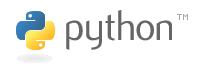
\includegraphics[width=0.5\textwidth]{img/python-logo.png}
	\end{figure}
	
	Python ist sehr \emph{einfach} zu lernen und deswegen auch gut für Programmieranfänger geeignet. Dabei kann es \emph{kostenlos heruntergeladen} werden und wird für alle gängigen Betriebssysteme angeboten.
	
	\subsection*{Python unter Windows installieren}
	\begin{enumerate}
		\item \emph{Öffne die Seite \url{http://python.org/download/}}. Leider gibt es diese Seite nur auf englisch. Wenn du bei den nächsten Schritten Probleme hast, frage doch mal deine Eltern oder Freunde, ob sie dir weiterhelfen können.
		
		\item Wir arbeiten mit Python 3. Wenn du ein 64-Bit-System benutzt, dann lade die Datei \enquote{\emph{Python 3.2.2 Windows X86-64 MSI Installer}} herunter. Wenn nicht, oder wenn du dir nicht sicher bist, dann lade die Datei \enquote{\emph{Python 3.2.2 Windows x86 MSI Installer}} herunter.
		
		\item Danach kannst du Python mit einem Doppelklick auf die heruntergeladene Datei installieren. Es öffnet sich ein \emph{Installationsdialog} – du kannst alle Einstellungen so lassen und auf \enquote{next} klicken. Wenn du nicht als Administrator angemeldet bist, kann es sein, dass du von Windows nach dem Administrator-Passwort gefragt wirst. Gib es ein oder frage denjenigen, dem der Computer gehört, ob er es eingeben kann. Danach installiert sich Python fertig und du kannst auf \enquote{finish} klicken.
		
		\item Im Windows-Startmenü taucht jetzt ein Programm mit dem Namen \enquote{\emph{IDLE (Python GUI)}} auf. Klicke darauf, um die Python-Shell zu starten und mit dem Programmieren loszulegen!
	\end{enumerate}
	
	\subsection*{Hilfe beim Programmieren lernen}
	Weil Python kostenlos verfügbar ist und von so vielen Programmierern benutzt wird, gibt es im Internet besonders viele \emph{Wikis, Foren, Anleitungen und sogar ganze Bücher}. So bekommt man viel Hilfe beim Lernen – vom ersten Befehl bis hin zu komplizierten Programmen.
	
	\begin{enumerate}
		\item Ein komplettes \emph{offizielles Tutorial} in deutsch gibt es unter \url{http://tutorial.pocoo.org/}. Wenn du Python schon installiert hast, kannst du gleich mit dem dritten Kapitel \enquote{\emph{Eine informelle Einführung in Python}} loslegen. Ab hier werden die wichtigsten Dinge, die man zum Programmieren braucht, Schritt für Schritt erklärt. Die Original-Version in englisch findest du unter \url{http://docs.python.org/py3k/tutorial/index.html}.
		
		\item Gleich ein ganzes \emph{Buch extra für Kids} (\enquote{Schlangengerangel für
Kinder}) kannst du dir unter \url{https://code.google.com/p/swfk-de/downloads/list} herunterladen.
		
		\item Jeder lernt anders. Falls du mit digitalen Büchern nichts anfangen kannst, sondern lieber eins aus Papier möchtest, gibt es da zum Beispiel noch \enquote{\emph{Python für Kids}} von Gregor Lingl oder \enquote{\emph{Hello World!: Programmieren für Kids und andere Anfänger}} von Warren D. Sande.
		
		\item Wenn du gut genug \emph{Englisch} verstehst, kannst du mit den beiden Büchern unter \url{http://inventwithpython.com/} super lernen, \emph{Spiele in Python zu programmieren}. Beide Bücher kann man entweder als \enquote{echtes} Buch kaufen oder kostenlos online lesen (oder beides). Außerdem gibt es auf der Website noch die Quelltexte der Spiele zum Herunterladen, Videos und andere nützliche Sachen.
		
	\end{enumerate}
	
	
\end{document}